\documentclass[resume]{subfiles}


\begin{document}
    \section{Intégration numérique}
	\subsection{Formule du trapèze}
	$$\boxed{\int_{a}^{b}f(x)dx\approx \frac{b-a}{2}\left(f(a)+f(b)\right)}$$
	\subsection{Formule composite du trapèze}
Formule du trapèze avec sous-division ($n$ intervalles)
$$h=\frac{b-a}{n}$$
$$\boxed{\int_{a}^{b}f(x)dx\approx h\left(\frac{1}{2}f(a)+\sum_{j=1}^{n-1}f(x_j)+\frac{1}{2}f(b)\right)}$$
	\subsection{Formule du point milieu}
	$$\boxed{M=h\left(f(x_{0.5})+f(x_{1.5})+\cdots+f(x_{n-0.5 })\right)}$$
	$$T\left(\frac{h}{2}\right)=\frac{1}{2}\left(T(h)+M(h)\right)$$
	\subsubsection{Algorithme pour $n=4$}
	\begin{enumerate}
	\item $h=b-a$
	\item $T(h)=\frac{h}{2}\left(f(x_0)+f(x_4)\right)$
	\item $M(h)=hf(x_2)$
	\item $T\left(\frac{h}{2}\right)=\frac{1}{2}\left(M(h)+T(h)\right)$
	\item $M\left(\frac{h}{2}\right)=\frac{h}{2}\left(f(x_1)+f(x_3)\right)$
	\item $T\left(\frac{h}{4}\right)=\frac{1}{2}\left(M\left(\frac{h}{2}\right)+T\left(\frac{h}{2}\right)\right)$
	\end{enumerate}
	\subsubsection{Erreur}
	$$\abs{\int_a^bf(x)dx-T(h)}\leq \frac{h^2(b-a)}{12}\max_{a\leq x\leq b}\abs{f''(x)}$$
	Optimal si
	\begin{enumerate}
	\item La fonction est \textbf{périodique}
	\item La fonction est \textbf{infiniment dérivable}
	\item On intègre sur une période
	\end{enumerate}
	\subsection{Méthode de Simpson}
	$$\boxed{\int_a^{b}f(x)dx\approx \frac{h}{3}\left(f(a)+4f\left(\frac{a+b}{2}\right)+f(b)\right)}$$
	$$h=\frac{b-a}{2}$$
	\subsubsection{Erreur}
	$$\abs{\int_a^bf(x)dx-S}\leq \frac{h^5}{90}\max_{a\leq x\leq b}\abs{f^{(4)}(x)}$$
	\subsection{Formule de Newton-Cotes}
	Avec $n=3$ (3/8 de Simpson)
	$$\int_{x_0}^{x_3}f(x)dx\approx \frac{3h}{8}\left(f(x_0)+3f(x_1)+3f(x_2)+f(x_3)\right)$$
	\begin{align*}
	\int_{x_0}^{x_4}f(x)dx\approx \frac{2h}{45} \Big(7f(x_0)&+32f(x_1)+12f(x_2)\\ &+32f(x_3)+7f(x_4)\Big)
	\end{align*}
	
	
	$n$ pair : polynômes jusqu'à $n+1$. $n$ impair : polynômes jusqu'à $n$
	\subsection{Formule de composition de Simpson}
	Cas général avec $2n$ sous intervalles
	$$\boxed{\begin{split}S_c=\frac{h}{3}\Big(f(a)&+3f(x_1)\\&+f(b)+2\sum_{k=1}^{n-1}\left(f(x_{2k})+2f(x_{2k+1})\right)\Big)\end{split}}$$
	\subsubsection{Erreur}
	$$\boxed{\abs{\int_a^bf(x)dx-S_c}\leq \frac{h^4(b-a)}{180}\max_{a\leq x\leq b}\abs{f^{(4)}(x)}}$$
	$$h=\frac{b-a}{2n}$$
	\subsection{Formule de Simpson adaptative}
	Intervalles non uniformes
	\subsection{Récapitulatif}
	\begin{figure}[H]
	\centering
	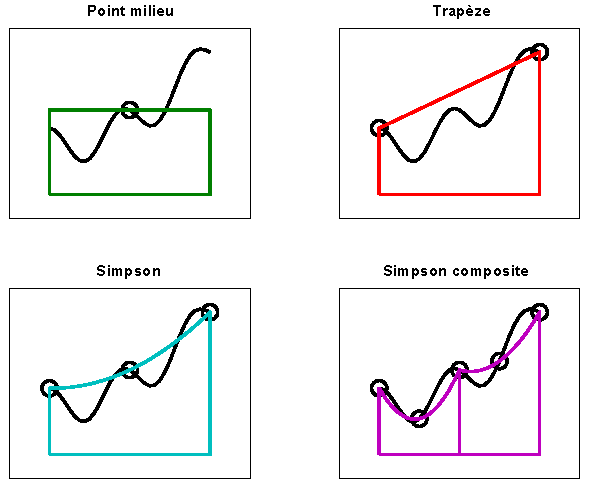
\includegraphics[width=\columnwidth]{img_8.pdf}
	\end{figure}

    
\end{document}